\documentclass[12pt, letterpaper]{article}

% Page layout and spacing
\usepackage[margin=1in]{geometry}
\usepackage{setspace}
\usepackage{float}
\doublespacing

% Mathematical and scientific packages
\usepackage{amsmath, amssymb}
\usepackage{subcaption}
\usepackage{booktabs}
\usepackage[hidelinks]{hyperref}
\usepackage{graphicx}

\setlength{\emergencystretch}{2em}
\graphicspath{{plots/}{./}}

\title{Analytical and Numerical Stability Analysis of the Lagrange Points in the Restricted Three-Body Problem}
\author{Kalel Chester}
\date{November, 2026}

\begin{document}

\maketitle

\begin{abstract}
The circular restricted three-body problem models the motion of a massless test particle under the gravitational influence of two massive primary bodies moving in circular orbits about their common center of mass. Although the general system exhibits chaotic dynamics, five stationary equilibrium configurations---the Lagrange points ($L_1$--$L_5$)---exist in the co-rotating reference frame. In this paper, we derive the locations of the collinear ($L_1, L_2, L_3$) and triangular ($L_4, L_5$) equilibrium points from the co-rotating effective potential and evaluate the relative error of first-order small-mass-ratio approximations against numerical root-finding solutions obtained via \texttt{scipy.optimize.\allowbreak fsolve}. Because the co-rotating effective potential contains a velocity-dependent Coriolis term, we assess equilibrium stability through linear perturbation analysis rather than potential curvature alone, computing the eigenvalues and characteristic $e$-folding times of each point. Analytically, $L_1$, $L_2$, and $L_3$ are unstable saddle points for all mass ratios, whereas $L_4$ and $L_5$ achieve linear stability when $M_1 / M_2 \ge \frac{1}{2}(25 + 3\sqrt{69}) \approx 24.96$. Finally, we validate these analytical predictions through direct $N$-body integrations in \texttt{REBOUND} using the 15th-order adaptive Gauss--Radau integrator \texttt{IAS15} at mass ratios $M_1/M_2 = 10$ and $M_1/M_2 = 25$, confirming exponential departure from unstable configurations and long-term boundedness at the stable Trojan points.
\end{abstract}

\section{Introduction}

The restricted three-body problem is a foundational model in classical mechanics that describes the dynamics of a small, effectively massless test particle moving under the gravitational attraction of two much larger bodies, $M_1$ and $M_2$. For generic initial conditions, the trajectories of the test particle are non-integrable and exhibit chaotic behavior. Nevertheless, when viewed in a reference frame co-rotating with the two primary masses, there exist five special equilibrium configurations---known as the Lagrange points---at which the gravitational forces of the two primaries and the centrifugal force of the rotating frame balance exactly, allowing the test particle to remain stationary relative to the two larger bodies \cite{cornish}.

Understanding the locations and stability properties of these equilibria is of direct physical relevance to astrodynamics and space mission design. Despite the linear instability of the collinear points $L_1$ and $L_2$, spacecraft can exploit bounded oscillatory eigenmodes in the full three-dimensional system to occupy periodic and quasi-periodic halo and Lissajous orbits with minimal propellant expenditure. Notable examples include the James Webb Space Telescope (JWST) stationed near the Sun--Earth $L_2$ point \cite{petersen} and the Solar and Heliospheric Observatory (SOHO) operating near the Sun--Earth $L_1$ point \cite{roberts}. Conversely, when the primary mass ratio exceeds a critical threshold, the triangular points $L_4$ and $L_5$ (referred to as Trojan points) become linearly stable, permitting long-term natural trapping of minor bodies in systems such as Sun--Earth and Earth--Moon \cite{cornish}.

The objective of this project is threefold: (i) to derive the positions of all five Lagrange points analytically and compare small-mass-ratio approximations against exact numerical solutions, (ii) to determine the linear stability and characteristic divergence timescales of each equilibrium point, and (iii) to numerically simulate the perturbed dynamics of test particles placed at each Lagrange point to validate the analytical stability criteria.

\section{Analytical Formulation}

\subsection{Effective Potential and Equations of Motion}

Following the derivation of Cornish \cite{cornish}, consider two primary bodies of masses $M_1$ and $M_2$ located at position vectors $\vec{r}_1$ and $\vec{r}_2$, respectively, separated by a fixed distance $R$. The gravitational force exerted on a third test mass $m$ at position $\vec{r}$ is
$$ 
\vec{F}
= -\frac{GM_1m}{|\vec{r}-\vec{r_1}|^3} (\vec{r}-\vec{r_1})
-\frac{GM_2m}{|\vec{r}-\vec{r_2}|^3} (\vec{r}-\vec{r_2})
$$
where $G$ is the universal gravitational constant. To identify stationary configurations, we transform into a co-rotating reference frame whose origin lies at the center of mass of $M_1$ and $M_2$ and which rotates at the constant angular frequency $\Omega$ determined by Kepler's third law:
$$
\Omega^2 R^3 = G(M_1 + M_2).
$$
Setting the test particle mass $m = 1$ without loss of generality, the effective potential in the co-rotating frame is given by
\begin{equation}
U_\Omega = U - 
\vec{v} \cdot (\vec{\Omega} \times \vec{r}) -
\frac{1}{2}(\vec{\Omega} \times \vec{r})\cdot(\vec{\Omega} \times \vec{r}),
\label{eq:ueff}
\end{equation}
where $\vec{v}$ is the velocity of the test particle in the rotating frame and $U$ is the Newtonian gravitational potential,
$$
U = -G\left(\frac{M_1}{|\vec{r} - \vec{r}_1|} + \frac{M_2}{|\vec{r} - \vec{r}_2|}\right).
$$
The velocity-dependent Coriolis term $-\vec{v} \cdot (\vec{\Omega} \times \vec{r})$ vanishes for stationary points ($\vec{v} = \vec{0}$) and therefore does not affect the positions of the Lagrange points, although it plays a decisive role in their dynamical stability.

Defining the dimensionless mass fractions
$$
\alpha = \frac{M_2}{M_1 + M_2}, \qquad \beta = \frac{M_1}{M_1 + M_2},
$$
the two primaries lie on the $x$-axis at $(-\alpha R, 0)$ and $(\beta R, 0)$ in the center-of-mass frame. Taking the negative gradient of the static part of Eq.~\eqref{eq:ueff} yields the effective force on a stationary test particle in the orbital plane:
\begin{equation}
\vec{F} = \Omega^2
\begin{pmatrix}
x - \dfrac{\beta(x + \alpha R)R^3}{\left((x + \alpha R)^2 + y^2\right)^{3/2}} - \dfrac{\alpha(x - \beta R)R^3}{\left((x - \beta R)^2 + y^2\right)^{3/2}} \\[14pt]
y - \dfrac{\beta y R^3}{\left((x + \alpha R)^2 + y^2\right)^{3/2}} - \dfrac{\alpha y R^3}{\left((x - \beta R)^2 + y^2\right)^{3/2}}
\end{pmatrix}.
\label{eq:feff}
\end{equation}

\subsection{Identification of the Collinear Points (\texorpdfstring{$L_1, L_2, L_3$}{L1, L2, L3})}

By symmetry about the $x$-axis, the $y$-component of the effective force vanishes identically along $y = 0$. Setting $y = 0$ and introducing the dimensionless coordinate transformation $x = R(u + \beta)$, the equilibrium condition $F_x = 0$ reduces to three quintic polynomial equations \cite{cornish}:
$$
u^2\left((1 - s_1) + 3u + 3u^2 + u^3\right) = \alpha\left(s_0 + 2s_0 u + (1 + s_0 - s_1)u^2 + 2u^3 + u^4\right),
$$
where $s_0 = \operatorname{sign}(u)$ and $s_1 = \operatorname{sign}(u + 1)$. The sign pairs $(s_0, s_1) = (-1, 1)$, $(1, 1)$, and $(-1, -1)$ correspond to $L_1$, $L_2$, and $L_3$, respectively, and each quintic possesses a unique real root.

Because no closed-form algebraic solution exists for arbitrary $\alpha$, we expand the roots in the astrophysically relevant limit $\alpha \ll 1$, which holds strongly for the Sun--Earth system ($\alpha \approx 10^{-6}$) and more modestly for the Earth--Moon system ($\alpha \approx 10^{-2}$). To leading order in $\alpha$, the collinear Lagrange points are located at \cite{cornish}:
\begin{equation}
L_1: \begin{pmatrix} R\left[1 - \left(\dfrac{\alpha}{3}\right)^{1/3}\right] \\ 0 \end{pmatrix}, \quad
L_2: \begin{pmatrix} R\left[1 + \left(\dfrac{\alpha}{3}\right)^{1/3}\right] \\ 0 \end{pmatrix}, \quad
L_3: \begin{pmatrix} -R\left[1 + \dfrac{5}{12}\alpha\right] \\ 0 \end{pmatrix}.
\label{eq:collinear_approx}
\end{equation}

\subsection{Identification of the Triangular Points (\texorpdfstring{$L_4, L_5$}{L4, L5})}

To locate the off-axis equilibria ($y \neq 0$), we resolve the effective force into components perpendicular and parallel to the position vector $\vec{r}$ \cite{cornish}. The perpendicular component is
$$
F_\Omega^\perp = \alpha \beta y \Omega^2 R^3 \left( \frac{1}{\left((x - \beta R)^2 + y^2\right)^{3/2}} - \frac{1}{\left((x + \alpha R)^2 + y^2\right)^{3/2}} \right).
$$
For $y \neq 0$, setting $F_\Omega^\perp = 0$ requires that the test particle be equidistant from $M_1$ and $M_2$. Substituting this condition into the parallel force component yields
$$
F_\Omega^\parallel = \Omega^2 \frac{x^2 + y^2}{R} \left( \frac{1}{R^3} - \frac{1}{\left((x - \beta R)^2 + y^2\right)^{3/2}} \right).
$$
Setting $F_\Omega^\parallel = 0$ establishes that the test particle must lie at distance $R$ from each primary mass, forming the third vertex of an equilateral triangle of side length $R$ with $M_1$ and $M_2$:
\begin{equation}
L_4: \begin{pmatrix} \dfrac{R}{2}(\beta - \alpha) \\[6pt] \dfrac{\sqrt{3}}{2}R \end{pmatrix}, \qquad
L_5: \begin{pmatrix} \dfrac{R}{2}(\beta - \alpha) \\[6pt] -\dfrac{\sqrt{3}}{2}R \end{pmatrix}.
\label{eq:triangular_exact}
\end{equation}
Unlike Eq.~\eqref{eq:collinear_approx}, the coordinates of $L_4$ and $L_5$ in Eq.~\eqref{eq:triangular_exact} are exact for all mass ratios.

\subsection{Linear Stability Analysis}

Because the effective potential in Eq.~\eqref{eq:ueff} depends on velocity through the Coriolis term, the local curvature of the static effective potential alone cannot determine stability. Instead, we linearize the equations of motion around each equilibrium point $(x_i, y_i)$ by introducing small perturbations:
$$
x = x_i + \delta x, \quad y = y_i + \delta y, \quad v_x = \delta v_x, \quad v_y = \delta v_y.
$$
Defining the perturbation state vector $\vec{\xi} = (\delta x, \delta y, \delta v_x, \delta v_y)^T$, the linearized equations of motion take the matrix form
\begin{equation}
\frac{d}{dt}
\begin{pmatrix} \delta x \\ \delta y \\ \delta v_x \\ \delta v_y \end{pmatrix}
=
\begin{pmatrix}
0 & 0 & 1 & 0 \\
0 & 0 & 0 & 1 \\
-\dfrac{\partial^2 U_\Omega}{\partial x^2} & -\dfrac{\partial^2 U_\Omega}{\partial x \partial y} & 0 & 2\Omega \\
-\dfrac{\partial^2 U_\Omega}{\partial y \partial x} & -\dfrac{\partial^2 U_\Omega}{\partial y^2} & -2\Omega & 0
\end{pmatrix}
\begin{pmatrix} \delta x \\ \delta y \\ \delta v_x \\ \delta v_y \end{pmatrix},
\label{eq:linearized}
\end{equation}
where all second partial derivatives of $U_\Omega$ are evaluated at $(x_i, y_i)$.

The general solution is a superposition of eigenmodes, $\vec{\xi}(t) = \sum_{k=1}^4 c_k e^{\lambda_k t}$. Writing each eigenvalue as $\lambda = \gamma + i\omega$, the general solution becomes $\vec{\xi}(t) = \sum_{k=1}^4 c_k e^{\gamma_k t}e^{i\omega_k t}.$ The imaginary part of the eigenvalue corresponds to oscillatory motion, while the real part determines the exponential growth or decay. The equilibrium is unstable whenever any eigenvalue has a positive real part $\gamma = \operatorname{Re}(\lambda) > 0$. The rate of exponential divergence (in the case $\gamma > 0$) is quantified by the characteristic $e$-folding time,
$$
\tau = \frac{1}{\gamma},
$$
which represents the time required for a small initial displacement along the unstable eigenmode to grow by a factor of $e$. In the case of a negative real eigenvalue, $\tau$ represents the time required for a small initial displacement along the stable eigenmode to decay by a factor of $e$. Lastly, if all eigenvalues are purely imaginary, the equilibrium is linearly stable and $\tau \to \infty$.

\subsubsection{Stability of \texorpdfstring{$L_1$ and $L_2$}{L1 and L2}.}
Near $L_1$ and $L_2$, the static effective potential forms a saddle point with curvatures (for $\alpha \ll 1$)
$$
\frac{\partial^2 U_\Omega}{\partial x^2} = -9\Omega^2, \qquad
\frac{\partial^2 U_\Omega}{\partial y^2} = 3\Omega^2, \qquad
\frac{\partial^2 U_\Omega}{\partial x \partial y} = \frac{\partial^2 U_\Omega}{\partial y \partial x} = 0.
$$
The resulting eigenvalues of Eq.~\eqref{eq:linearized} are
$$
\lambda = \pm \Omega \sqrt{1 + 2\sqrt{7}}, \qquad \pm i\Omega \sqrt{2\sqrt{7} - 1}.
$$
The presence of a positive real eigenvalue renders both $L_1$ and $L_2$ linearly unstable, with an $e$-folding time of $\tau \approx \frac{2}{5\Omega} \approx 23\text{ days}$ for the Sun--Earth system \cite{cornish}. Consequently, an uncorrected spacecraft placed at $L_1$ or $L_2$ will drift away within a few months. In practice, however, missions such as JWST at $L_2$ \cite{petersen} and SOHO at $L_1$ \cite{roberts} inject into periodic or quasi-periodic halo and Lissajous orbits associated with the purely imaginary eigenvalue pair $\pm i\Omega\sqrt{2\sqrt{7}-1}$ so that the initial component along the unstable eigenmode is nearly zero. Small periodic station-keeping maneuvers---performed every few weeks for JWST \cite{petersen} and roughly every 90 days for SOHO \cite{roberts}---then cancel unstable mode excitations caused by solar radiation pressure, planetary perturbations and other perturbations.

\subsubsection{Stability of \texorpdfstring{$L_3$}{L3}.}
The collinear point $L_3$ is likewise a saddle point, with curvatures to first order in $\alpha$ given by
$$
\frac{\partial^2 U_\Omega}{\partial x^2} = -\frac{1}{4}(12 + 7\alpha)\Omega^2, \qquad
\frac{\partial^2 U_\Omega}{\partial y^2} = \frac{7\alpha \Omega^2}{8}, \qquad
\frac{\partial^2 U_\Omega}{\partial x \partial y} = \frac{\partial^2 U_\Omega}{\partial y \partial x} = 0.
$$
The eigenvalues to first order in $\alpha$ are
$$
\lambda = \pm \frac{i}{8}(8 + 7\alpha)\Omega, \qquad \pm \frac{1}{2}\sqrt{\frac{21\alpha}{2}}\,\Omega.
$$
Because a positive real eigenvalue exists, $L_3$ is unstable, though its divergence is much slower than at $L_1$ and $L_2$, yielding $\tau \approx 56.7\text{ years}$ for the Sun--Earth system \cite{cornish}.

\subsubsection{Stability of \texorpdfstring{$L_4$ and $L_5$}{L4 and L5}.}
At the triangular points $L_4$ and $L_5$, the second derivatives of the effective potential are
$$
\frac{\partial^2 U_\Omega}{\partial x^2} = -\frac{3}{4}\Omega^2, \qquad
\frac{\partial^2 U_\Omega}{\partial y^2} = -\frac{9}{4}\Omega^2, \qquad
\frac{\partial^2 U_\Omega}{\partial x \partial y} = \frac{\partial^2 U_\Omega}{\partial y \partial x} = \pm \frac{3\sqrt{3}}{4}\kappa\Omega^2,
$$
where $\kappa = (M_1 - M_2)/(M_1 + M_2) = 1 - 2\alpha$. Solving the characteristic equation of Eq.~\eqref{eq:linearized} yields
$$
\lambda = \pm i \frac{\Omega}{2}\sqrt{2 \pm \sqrt{27\kappa^2 - 23}}.
$$
Linear stability requires all four eigenvalues to be purely imaginary, which holds if and only if \cite{cornish}
$$
\kappa^2 > \frac{23}{27} \qquad \text{and} \qquad \sqrt{27\kappa^2 - 23} \le 2. 
$$
Since $\kappa < 1$, the second inequality is always satisfied, while the first yields requirement that the mass ratio of the two primaries exceed a critical threshold:
\begin{equation}
M_1 \ge \frac{1}{2}M_2\left(25 + 3\sqrt{69}\right) \approx 24.96\, M_2.
\label{eq:trojan_condition}
\end{equation}
When Eq.~\eqref{eq:trojan_condition} is satisfied---as in both the Sun--Earth and Earth--Moon systems---the Coriolis force stabilizes motion about the potential maxima at $L_4$ and $L_5$, producing stable Trojan orbits.

\section{Numerical Methodology}

All numerical calculations and visualizations were implemented in Python using \texttt{NumPy} \cite{numpy}, \texttt{SciPy} \cite{scipy}, \texttt{Matplotlib} \cite{matplotlib}, \texttt{Seaborn} \cite{seaborn}, and the \texttt{REBOUND} $N$-body library \cite{rebound}.

\subsection{Potential Visualization and Root Finding}

To visualize the effective potential and force fields, a baseline model system was defined in arbitrary dimensionless units with $G = 1$, $M_1 = 10$, $M_2 = 1$ ($M_1/M_2 = 10$), primary separation $R = 10$, and $\vec{v} = \vec{0}$. The effective potential $U_\Omega(x, y)$ and numerical gradient magnitude $|\vec{F}| = |\nabla U_\Omega|$ were evaluated across a Cartesian grid spanning $x \in [-16, 16]$ and $y \in [-12, 12]$. Exact numerical coordinates of all five Lagrange points were obtained by solving $\vec{F}(x, y) = \vec{0}$ from Eq.~\eqref{eq:feff} using \texttt{scipy.optimize.fsolve} \cite{scipy} seeded with analytical initial guesses near each equilibrium.

To quantify the validity of the $\alpha \ll 1$ collinear approximations in Eq.~\eqref{eq:collinear_approx}, we performed a logarithmic sweep over mass ratios $\alpha/\beta \in [10^{-10}, 1)$ in increments of 0.1 (setting $M_2 = 1$ and $M_1 = \beta/\alpha$). At each mass ratio, the relative position error was computed as
$$
\epsilon_i = \frac{\|\vec{r}_{i,\text{exact}} - \vec{r}_{i,\text{approx}}\|}{\|\vec{r}_{i,\text{exact}}\|},
$$
where $\vec{r}_{i,\text{exact}}$ is the numerical root returned by \texttt{fsolve}.

\begin{figure}[htbp]
\centering
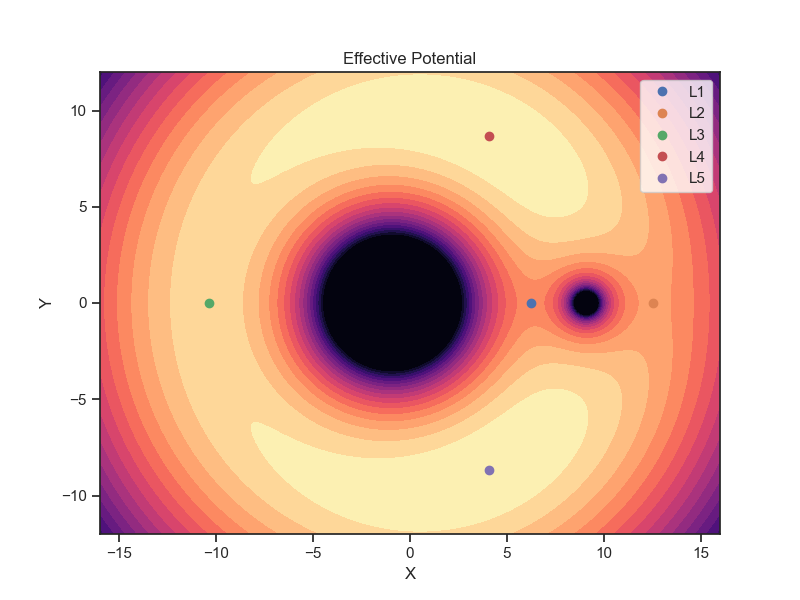
\includegraphics[width=0.8\textwidth]{ueff}
\caption{Effective potential $U_\Omega(x, y)$ (clamped below at $-3$ for visual contrast) for $M_1 = 10$, $M_2 = 1$, $R = 10$, $G = 1$, and $\vec{v} = \vec{0}$, with the numerically calculated Lagrange points $L_1$--$L_5$ labeled.}
\label{fig:ueff}
\end{figure}

\begin{figure}[htbp]
\centering
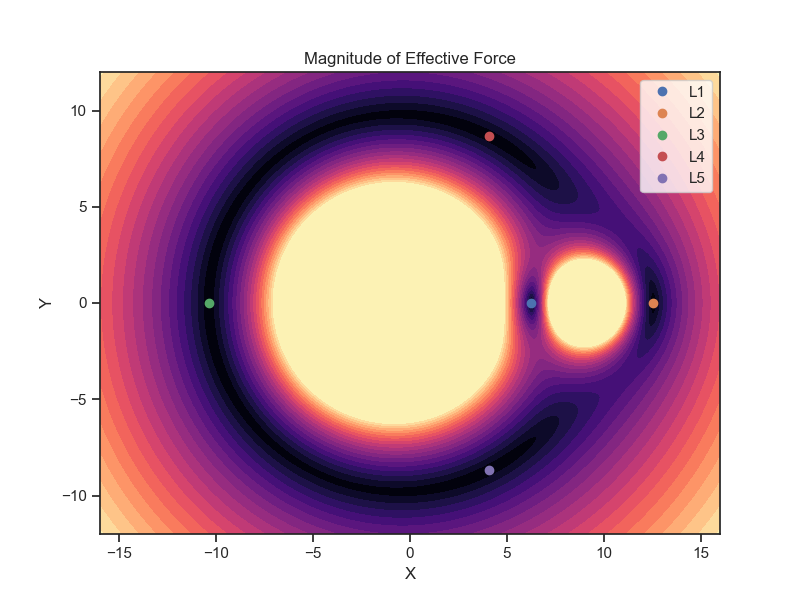
\includegraphics[width=0.8\textwidth]{feff}
\caption{Magnitude of the co-rotating effective force $|\vec{F}| = |\nabla U_\Omega|$ corresponding to the effective potential in Fig.~\ref{fig:ueff}, showing vanishing force at all five Lagrange points.}
\label{fig:feff}
\end{figure}

\subsection{\texorpdfstring{$N$}{N}-Body Perturbation Simulations}

Dynamical stability was tested directly in \texttt{REBOUND} \cite{rebound} using the \texttt{IAS15} integrator, an adaptive 15th-order Gauss--Radau scheme accurate to machine precision over long orbital timescales \cite{ias15}. The two primary bodies were initialized on circular orbits in the center-of-mass frame with angular velocity $\Omega = \sqrt{G(M_1 + M_2)/R^3}$, and massless test particles ($m = 0$) were placed at the numerically calculated Lagrange point coordinates with matching velocities $(v_x, v_y) = (-\Omega y_i, \Omega x_i)$.

For each Lagrange point, a small randomized perturbation was added to the initial $(x, y)$ coordinates of the test particle (sampled from a zero-mean Gaussian distribution in the simulation script, with a maximum of $10^{-4}$ in dimensionless units). The system was integrated forward in steps of $\Delta t = 0.1$ over $20{,}000$ steps, applying a frame rotation of angle $-\Omega \Delta t$ about the $z$-axis at each step to visualize trajectories in the co-rotating frame. To test the analytical stability boundary of Eq.~\eqref{eq:trojan_condition}, simulations were performed first at the unstable baseline ratio $M_1/M_2 = 10$ for all five Lagrange points, and then repeated for $L_4$ and $L_5$ at $M_1/M_2 = 25$, which just exceeds the critical threshold of $24.96$.

\section{Results and Discussion}

\subsection{Effective Potential, Force Field, and Approximation Error}

Figures~\ref{fig:ueff} and~\ref{fig:feff} display the effective potential $U_\Omega$ and effective force magnitude $|\vec{F}|$ for the baseline system ($M_1 = 10$, $M_2 = 1$, $R = 10$, $G = 1$) with the numerically computed Lagrange points overlaid. The exact numerical coordinates obtained from \texttt{fsolve} are summarized in Table~\ref{tab:lagrange_summary}. As expected from the analytical formulation, $L_1$, $L_2$, and $L_3$ sit at saddle points along the $x$-axis where $|\vec{F}| \to 0$, whereas $L_4$ and $L_5$ sit at local maxima of $U_\Omega$ forming equilateral triangles with the two primaries.

\begin{table}[htbp]
\centering
\singlespacing
\caption{Numerically computed Lagrange point coordinates for the baseline system ($G = 1$, $M_1 = 10$, $M_2 = 1$, $R = 10$) and corresponding analytical linear stability properties.}
\label{tab:lagrange_summary}
\begin{tabular}{lcccc}
\toprule
Point & $x$ & $y$ & Linear Stability & Sun--Earth $\tau$ \\
\midrule
$L_1$ & $6.266$   & $0.000$  & Unstable (saddle) & $\approx 23\text{ days}$ \\
$L_2$ & $12.561$  & $0.000$  & Unstable (saddle) & $\approx 23\text{ days}$ \\
$L_3$ & $-10.378$ & $0.000$  & Unstable (saddle) & $\approx 56.7\text{ years}$ \\
$L_4$ & $4.091$   & $8.660$  & Stable if $M_1/M_2 \ge 24.96$ & Stable (Trojan) \\
$L_5$ & $4.091$   & $-8.660$ & Stable if $M_1/M_2 \ge 24.96$ & Stable (Trojan) \\
\bottomrule
\end{tabular}
\end{table}

Figure~\ref{fig:mass_ratio_accuracy} shows the relative error of the first-order collinear approximations in Eq.~\eqref{eq:collinear_approx} as a function of mass ratio $\alpha/\beta$. For $L_1$ and $L_2$, the relative discrepancy decreases smoothly as a power law toward smaller mass ratios, falling below $10^{-3}$ for $\alpha/\beta \lesssim 10^{-3}$ (with a brief sign-crossing dip near $\alpha/\beta \approx 3 \times 10^{-3}$). The $L_3$ approximation converges even more rapidly, reaching the floating-point machine-precision floor ($\sim 10^{-16}$) for $\alpha/\beta \lesssim 10^{-5}$. Because Eq.~\eqref{eq:triangular_exact} is exact, $L_4$ and $L_5$ exhibit zero analytical approximation error across all mass ratios.

\begin{figure}[htbp]
\centering
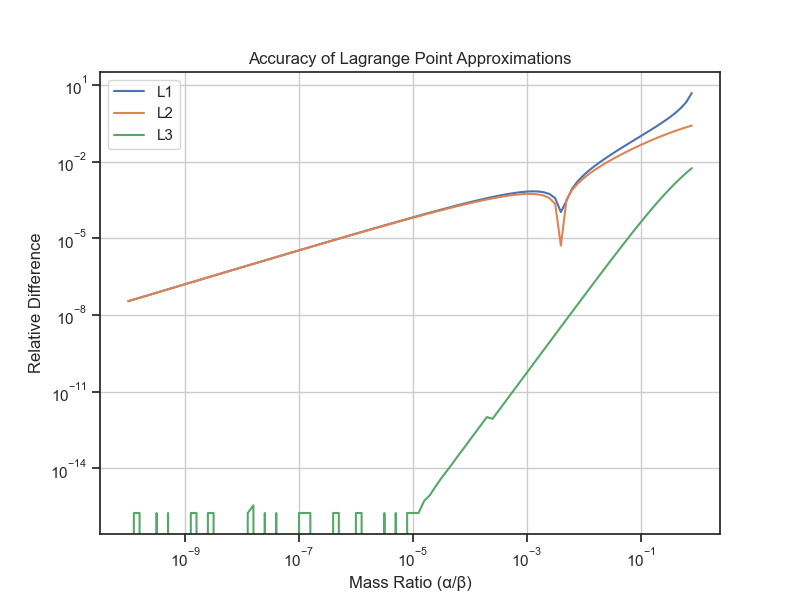
\includegraphics[width=0.78\textwidth]{mass_ratio_accuracy}
\caption{Relative difference between the first-order analytical approximations (Eq.~\eqref{eq:collinear_approx}) and exact numerical \texttt{fsolve} roots for $L_1$, $L_2$, and $L_3$ as a function of mass ratio $\alpha/\beta$.}
\label{fig:mass_ratio_accuracy}
\end{figure}

\subsection{Numerical Stability Simulations}

Direct \texttt{REBOUND}/\texttt{IAS15} integrations of perturbed test particles confirm the analytical linear stability predictions. At the baseline mass ratio $M_1/M_2 = 10$, which lies below the Trojan stability threshold of Eq.~\eqref{eq:trojan_condition}, test particles initialized with small position perturbations at $L_1$, $L_2$, $L_3$, $L_4$, and $L_5$ all depart from their equilibrium locations and enter unstable, chaotic trajectories in the co-rotating frame. Representative unstable configurations from the simulation suite are shown in Fig.~\ref{fig:unstable_dynamics_snapshots} and the stable configurations in Fig.~\ref{fig:stable_dynamics_snapshots} (full animated trajectories for $L_1$--$L_5$ are archived in the project repository).

\begin{figure}[htbp]
\centering
\begin{subfigure}[b]{0.48\textwidth}
    \centering
    \includegraphics[width=\textwidth]{l2}
    \caption{Perturbed $L_2$ ($M_1/M_2 = 10$)}
\end{subfigure}
\hfill
\begin{subfigure}[b]{0.48\textwidth}
    \centering
    \includegraphics[width=\textwidth]{l3}
    \caption{Perturbed $L_3$ ($M_1/M_2 = 10$)}
\end{subfigure}

\vspace{0.8em}

\begin{subfigure}[b]{0.48\textwidth}
    \centering
    \includegraphics[width=\textwidth]{l4}
    \caption{Perturbed $L_4$ ($M_1/M_2 = 10$)}
\end{subfigure}
\hfill
\begin{subfigure}[b]{0.48\textwidth}
    \centering
    \includegraphics[width=\textwidth]{l5}
    \caption{Perturbed $L_5$ ($M_1/M_2 = 10$)}
\end{subfigure}

\caption{Co-rotating frame snapshots from the \texttt{REBOUND}/\texttt{IAS15} perturbed test-particle simulations showing the larger primary (gold), secondary primary (blue), and perturbed test particle (orange). At $M_1/M_2 = 10$, all five Lagrange points are unstable.}
\label{fig:unstable_dynamics_snapshots}
\end{figure}

\begin{figure}[htbp]
\centering
\begin{subfigure}[b]{0.48\textwidth}
    \centering
    \includegraphics[width=\textwidth]{l4_heavy}
    \caption{Perturbed $L_4$ ($M_1/M_2 = 25$)}
\end{subfigure}
\hfill
\begin{subfigure}[b]{0.48\textwidth}
    \centering
    \includegraphics[width=\textwidth]{l5_heavy}
    \caption{Perturbed $L_5$ ($M_1/M_2 = 25$)}
\end{subfigure}

\caption{Co-rotating frame snapshots from the \texttt{REBOUND}/\texttt{IAS15} perturbed test-particle simulations showing the larger primary (gold), secondary primary (blue), and perturbed test particle (orange). At $M_1/M_2 = 25$, $L_4$ and $L_5$ are stable.}
\label{fig:stable_dynamics_snapshots}
\end{figure}
  

When the mass ratio is increased to $M_1/M_2 = 25$---just above the analytical stability boundary of $\frac{1}{2}(25 + 3\sqrt{69}) \approx 24.96$---perturbed test particles placed at $L_4$ and $L_5$ remain stably confined near the triangular equilibrium points for the full duration of the simulation, corresponding to more than $50{,}000$ orbits of the primary bodies. This numerical result directly validates both the stabilizing effect of the Coriolis force on the potential maxima at $L_4$ and $L_5$ and the sharp mass-ratio transition predicted by linear stability theory.

\section{Conclusion}

We have analyzed the positions and stability of the five Lagrange points in the circular restricted three-body problem using both analytical perturbation methods and high-precision numerical integration. The first-order small-mass-ratio approximations for the collinear points $L_1$, $L_2$, and $L_3$ agree closely with exact numerical roots for $\alpha/\beta \ll 1$, while $L_4$ and $L_5$ occupy exact equilateral-triangle configurations for all mass ratios. Linearizing the co-rotating equations of motion demonstrates that $L_1$, $L_2$, and $L_3$ are always unstable saddle points, whereas $L_4$ and $L_5$ become linearly stable for $\frac{M_1}{M_2} \ge \frac{1}{2}(25 + 3\sqrt{69}) \approx 24.96$. Direct $N$-body simulations using \texttt{REBOUND} and the \texttt{IAS15} integrator corroborate these predictions, exhibiting instability at all five points for $M_1/M_2 = 10$ and sustained orbital stability at $L_4$ and $L_5$ for $M_1/M_2 = 25$ over more than $50{,}000$ primary orbits.

\begin{thebibliography}{9}
\singlespacing

\bibitem{cornish}
N.~J. Cornish, \textit{The Lagrange Points}, NASA Technical Document, \url{https://science.nasa.gov/wp-content/uploads/2023/07/3322_lagrange.pdf}.

\bibitem{petersen}
J. Petersen, \textit{L2 Station Keeping Maneuver Strategy for the James Webb Space Telescope}, Preprint, \url{https://ntrs.nasa.gov/api/citations/20190028877/downloads/20190028877.pdf}.

\bibitem{roberts}
C.~E. Roberts, \textit{Long Term Missions at the Sun-Earth Libration Point L1: ACE, SOHO, and WIND}, AAS 11-485, \url{https://ntrs.nasa.gov/api/citations/20110022484/downloads/20110022484.pdf}.

\bibitem{rebound}
H. Rein and S.-F. Liu, ``REBOUND: an open-source multi-purpose N-body code for collisional dynamics,'' \textit{Astronomy \& Astrophysics}, vol. 537, A128, 2012, \url{https://doi.org/10.1051/0004-6361/201118085}.

\bibitem{ias15}
H. Rein and D.~S. Spiegel, ``IAS15: a fast, adaptive, high-order integrator for gravitational dynamics, accurate to machine precision over a billion orbits,'' \textit{Monthly Notices of the Royal Astronomical Society}, vol. 446, no. 2, pp. 1424--1437, 2015, \url{https://doi.org/10.1093/mnras/stu2164}.

\bibitem{numpy}
C.~R. Harris, K.~J. Millman, S.~J. van der Walt, et al., ``Array programming with NumPy,'' \textit{Nature}, vol. 585, pp. 357--362, 2020, \url{https://doi.org/10.1038/s41586-020-2649-2}.

\bibitem{scipy}
P. Virtanen, et al., ``SciPy 1.0: Fundamental Algorithms for Scientific Computing in Python,'' \textit{Nature Methods}, vol. 17, no. 3, pp. 261--272, 2020, \url{https://doi.org/10.1038/s41592-019-0686-2}.

\bibitem{matplotlib}
J.~D. Hunter, ``Matplotlib: A 2D Graphics Environment,'' \textit{Computing in Science \& Engineering}, vol. 9, no. 3, pp. 90--95, 2007.

\bibitem{seaborn}
M.~L. Waskom, ``seaborn: statistical data visualization,'' \textit{Journal of Open Source Software}, vol. 6, no. 60, 3021, 2021, \url{https://doi.org/10.21105/joss.03021}.

\end{thebibliography}

\end{document}